\subsection{Methods of Modelling Phages and Bacteria}
There are numerous ways to model the interactions between phages and bacteria.
Models can be built at a molecular level, where the model simulates the mechanical and chemical behavior of a phage as it interacts with the surface of a bacterium using computational chemistry methods.
On the other end of the spectrum, a different type of model can be built where populations of phages, bacteria, and resources can be modeled using Ordinary Differential Equations (ODEs) or Delay Differential Equations (DDEs).
DDEs are similar to ODEs, except where when ODEs are calculating the values of the equations at time $t$ using time $t-1$, DDEs can, but don't have to, use the value of the equation at time $t-\tau$, where $1 \leq \tau \leq t$. 
DDEs are a generalized version of ODEs. \newline 

Each type of system has its pros and cons.
With the molecular level model, the model is more complex and needs significantly more startup time, simulation time, and is in general much more complex.
However, more information can be gained from the simulations and can guide research in creating phages for a certain type of bacteria.
The ODE method is simpler and easier to set up, however it can only capture large population dynamics.
Certain assumptions about the community interactions have to be made.
For example, $\omega$ percent of the bacteria population is washed out.
The model can be made more complicated, by modelling each stage of the phage replication and lysis process, or instead of assuming exponential growth, there is a maximum carrying capacity of the population.
The model can be further altered by using a normally distributed variable $\textbf{N}(\mu=\omega, \sigma=1)$ to account for noise when measuring the data.
Ensuring the use of a seed value will ensure that each run of the model results in the same output. 

\subsubsection{Generalized Lotka-Voltera Model}
The Lotka-Voltera model, a first-order non-linear differential model, is a model that captures the dynamics between predators and prey, with phages being the predator and bacteria being the prey.
Any population can be modelled as such:
\[ 
    \frac{d{B}_i}{dt} = {B}_i \left(\left(r_i + \sum_{j}^{N} \alpha_{ij}{B}_j \right) - m_i\right)
\]
where $\cdots$.
 
\subsubsection{Generalized Consumer-Resource Model}
The generalized Consumer-Resource Model models the growth of a population and resource dynamics between a population of bacteria ${B}_i$ and a resource ${R}_i$. 
\begin{align}
    \frac{d{B}_i}{dt} &= r_i{B}_i \left(\sum_{\alpha} \Delta w_{i \alpha}C_{i \alpha}R_{\alpha}\right) - m_i {B}_i \\
    \frac{R_{\beta}}{dt} &= -\sum_i C_{i\beta}R_{\beta}{B_i} + \sum_{\alpha, i}D_{\beta\alpha}^{i}C_{i\alpha}R_{\beta}{B}_i \\
    \Delta w_{i\alpha} &= \sum_{\beta}D_{\beta \alpha}^{i}w_{\beta}
\end{align}

\subsubsection{Trait-Based Model}
The Trait-Based Model is a model that takes into account external factors such as the temperature or pH of the system and can be modeled as follows:  
\begin{align}
    \frac{dB_i}{dt} &= \left(r_i - m_i\right) B_i \\
    r_i &= \frac{r_{i\alpha}^{max}R_\alpha}{R_\alpha + K_{i\alpha}}e^{S_i\left(T-T_{ref}\right)}
\end{align}
where $S_i$ is the sensitivity to $B_i$ to factor $T$, and with trade off if $r_i^{max} > \text{ mean } r^{max} \text{ then } S_i > \text{ mean } S$. 

\subsubsection{Agent-Based Models}
Agent-based Models (ABM) model the system through space and time.
An $x \times y \times z$ grid (often $z$ is left out for a 2D system) is created and split into smaller subcells containing resources and microbes.
Each cell acts as its own tiny environment, where resources and microbes interact within the environment, but not with the neighboring cells.
Resources diffuse through the system using a PDE solver for a Boundary Value Problem (BVP).
Agents can move into neighboring grids with a probability $p$, where $p$ can depend on any number of parameters such as nutrient density, microbe density, or stochastic chance. \newline 
ABMs are useful when simulating many individual elements interacting in a system.
Chaotic or emergent behavior can arise from these interactions.
Chaotic behavior refers to the irregular and unpredictable evolution of a system's behavior due to nonlinear equations, exhibiting sensitive dependence on initial conditions \cite{encyclopedia_of_physical_science_and_technology}. \newline 
Emergent behavior is behavior that arises from the interactions of various agents in a system, that was not explicitly programmed into the system.
The behavior can be beneficial, neutral, or harmful, but it can not be predicted until it arises, \textit{if} it arises.
Agents can have simple rules, but when interacting with other agents, behavior that hasn't been programmed can arise.
Sometimes, people consider systems with emergent behaviors more complex than the sum of their parts. \newline
\begin{align} 
    \frac{\delta R_\alpha(r, t)}{\delta t} = \nabla \left[D \left( R_\alpha, r\right) \nabla R_\alpha \left( r, t \right) \right], r = \left(x, y\right)
\end{align}, where $r$ is a function of cell position $(x, y)$, and $t$ represents time. 
The cellular agents rules are as follows: 
\begin{align} 
    \frac{di}{dt} = r_i \left( \sum_\alpha \Delta w_{i\alpha}C_{i\alpha}R_\alpha\right)
\end{align}, where if $i> \text{ threshold, }\frac{i}{2}$ expands into the neighboring grid cell with a probability $p$. 
The system consumes resources and converts them into new sub-resource types with the following equation:
\begin{align}    
    \frac{dR_\alpha}{dt} &= -\sum_i C_{i\alpha}R_\alpha I \\
    \frac{dR_\beta}{dt} &= \sum_i C_{i\beta}R_\beta I + \sum_{\alpha, i}D_{\beta \alpha}^{i} C_{i \alpha} R_\alpha i
\end{align}. 

\subsection{Biology of Phages}
\subsubsection{What Are Phages?}

\subsubsection{How Does the Phage Cycle Work?}
There are 3 main parts to the phage-bacteria host cycle, the Infection stage, the Lysogenic cycle, and the Lytic cycle. 
In the infection stage, a phage floating through the environment detects and attaches to the surface of a bacteria cell. 
Once injected, the phage can control of the cell directly goes into the Lysogenic cycle or into the Lytic cycle. 
The phage proceeds to inject its DNA into the bacteria. 
\newline 

In the Lysogenic cycle, the phage DNA injects integrates into the genome of the bacteria. 
As the bacteria undergoes cellular replication, the DNA of the phage will be copied with the cell. 
After a set amount of time, the phage DNA can cut itself from the genome and enters the Lytic cycle.
\newline 

In the Lytic cycle, the phage hijacks the cellular process of the bacteria. 
The phage DNA hijacks the replication, transcription, and replication process of the cell, making more and more copies of phage. 
The phage parts build together to make a full part. 
Eventually the cell wall bursts releasing the phages into the environment ready to infect more bacteria. 

\paragraph{Infection Stage}
The infection stage is characterized as the searching for a bacterium, detection, and subsequent attachment and injection of DNA into the bacteria. 
\subparagraph{Attachment}


\subparagraph{Entry of Phage Into Bacteria}
Injection of DNA into bacteria. 

\paragraph{Lysogenic Cycle}
\subparagraph{Repression of DNA}
Represses DNA. 
\subparagraph{Integration of Phage DNA Into Bacteria DNA}
Integrate DNA. 
\subparagraph{Cellular Replication}
Cellular replication of the bacteria
\subparagraph{Induction of Phage}
Phage DNA leaved bacteria DNA. 

\paragraph{Lytic Cycle}
\subparagraph{Replication, Transcription, and Translation of the Phage DNA}
Replication of phage DNA. 
\subparagraph{Assembly of Phage Parts}
Assembly into a phage. 
\subparagraph{Lysis of the Bacterial Cell}
The lysis of the bacterial cell wall. 


\subsection{Bacterial Defense Against Phages} 
There is a constant battle between phages and bacteria. 
The bacteria don't want to be killed by the phages, so they adapt defenses such as thickening of the cell wall, or once the viral DNA has integrated with the bacteria's DNA, the bacteria will cut the viral DNA out of their DNA using CRISPR. 
\cite{iglerPhenotypicFluxRole2022}

\subsubsection{Mutations in Bacterial DNA (Genetic (Co-)Evolution)}
As bacteria cells grow and divide, random point mutations can occur in the DNA. 
These mutations can affect phage defenses, like thickening the cell wall or removing a receptor, making it harder for the phages to infect the bacteria cell. 
Mutations might not always work, however. 
They can be partially effective if full effectiveness requires multiple steps to achieve, which can occasionally fail \cite{lenskiTWOSTEPRESISTANCEESCHERICHIA1984} or the mutation brings a cost to the bacteria cell by losing receptors on the cell wall. \newline

Bacteria can horizontally transfer DNA to other bacteria on contact. 
There are three primary ways of this happening, which can be visualized in detail in \Cref{fig:horizontal_gene_transfer}. 

The first method is via conjugation, where a donor cell donates DNA fragments using a mechanism called the F-factor or plasmid with a pilus. 
The pilus on the donor cell connects to the recipient cell and the DNA can be transferred to the receiver cell. 

The second method, called transformation, occurs when a cell takes up DNA fragments released by a dead or degrading cell. 
Once inside the receiver cell, the donor DNA can integrate itself with the receiver DNA. 

The third method is via transduction. 
When a phage is assembling in the cell just before lysis, the phage can collect a piece of the hosts DNA instead of its own DNA. 
The dying bacterium proceeds to lyse, releasing the phages. 
The phage with the now dead hosts DNA can infect the next bacteria, injecting the DNA strand of the now dead cell into the new host cell. 
The old bacterial DNA will proceed to integrate with the new host cells DNA \cite{tamangHorizontalGeneTransfer2023}. 

\begin{figure}
    \centering
    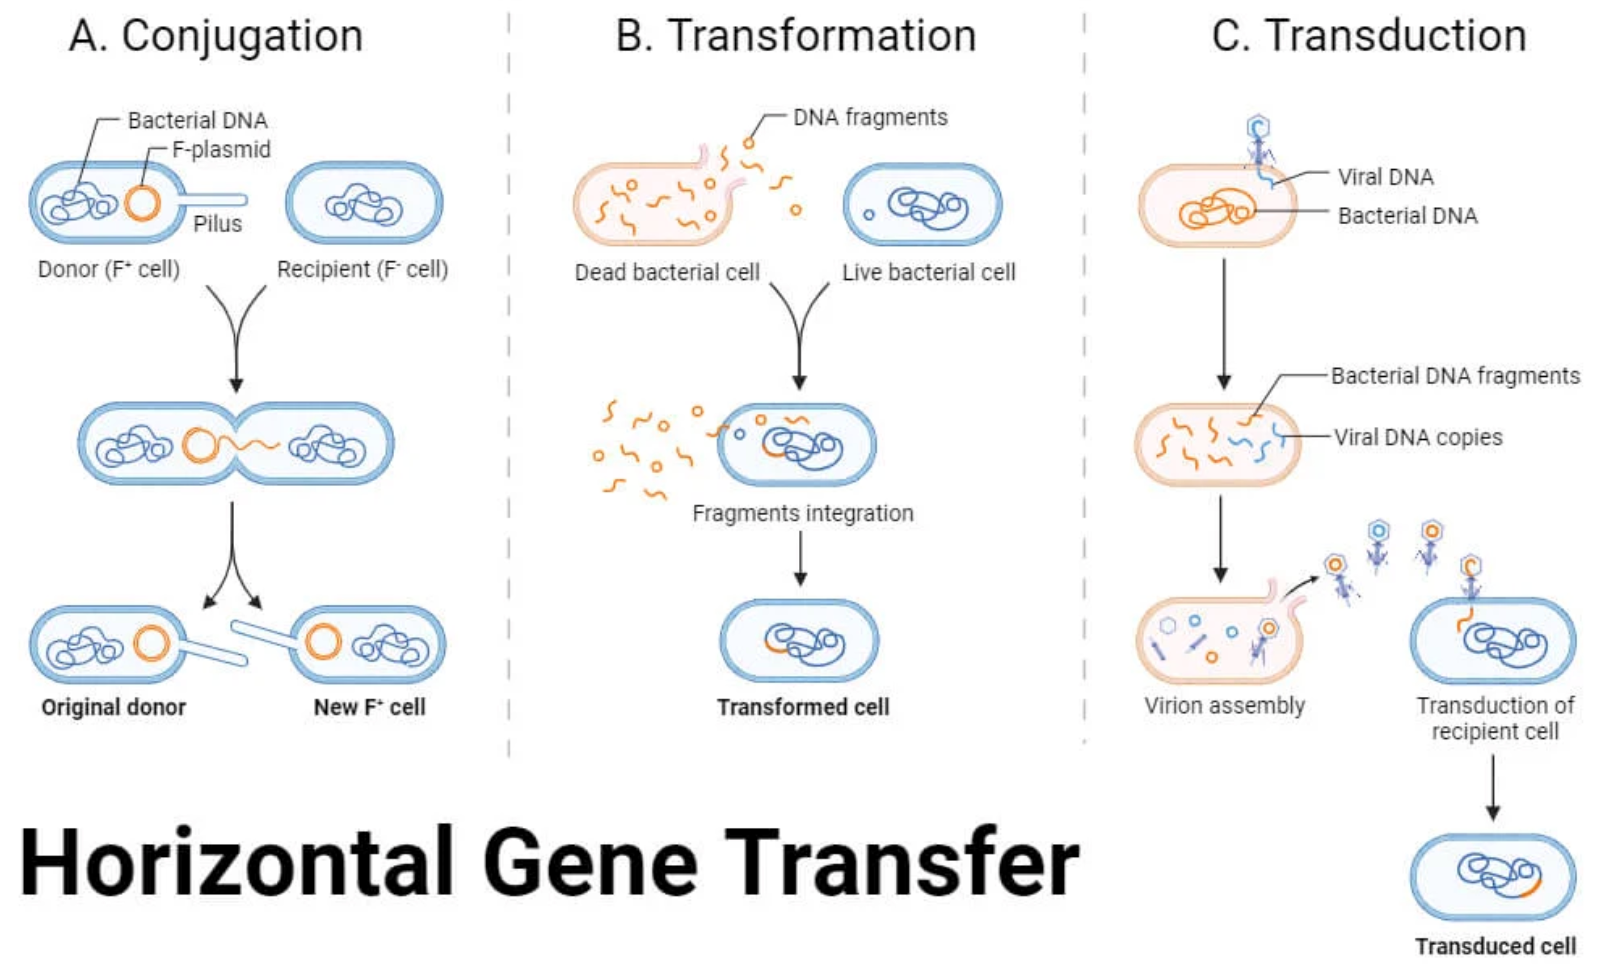
\includegraphics[width=0.7\linewidth]{Chapters/Figures/horizontal_gene_transfer.png}
    \caption{The three main ways that a (dead) bacterium can transfer DNA over to another bacterium \cite{tamangHorizontalGeneTransfer2023}.}
    \label{fig:horizontal_gene_transfer}
\end{figure}

\subsubsection{Phage Inactivation and Decoys}
Bacteria can further protect themselves by producing decoys that the phage will attach to instead of themselves, inactivating the phage. 
Freshly lysed bacteria can still contain biomarkers that phages use to detect the bacteria, but upon injection, nothing happens as the cell doesn't function anymore. 
Bacteria can also produce proteolytic enzymes that will damage the proteins found in a phage \cite{tanQuorumSensingDetermines2015}. 
Some bacteria can produce outer membrane vesicles that phages can absorb to, and later detach the vesicle with the phage \cite{rabinovitchBacterialDebrisEcological2003}. 
The vesicle will proceed to float away with the phage attached/injected inside, posing no risk to the source bacteria or to other bacteria. 
The impact of these vesicles acting as a sink is suspected to be minor \cite{bullPhageBacterialDynamicsSpatial2018}, but helpful nonetheless. 

\subsubsection{CRISPR-Cas Methods}
CRISPR is a gene editing tool that cells can use to cut out specified/unwanted parts of a DNA strand. 
Researchers are commonly using CRISPR to genetically engineer plants and animals to have specific features. 
Strands of DNA can be selectively added or removed from a DNA strand to achieve a better, more desired DNA strand. 
Specialized defenses in the bacteria can detect unwanted strands and remove the strand, acting as a line of defense against phages. 

\subsubsection{Phenotype Resistance}

\subsubsection{Spatial Refuge/Biofilms} 
Usually bacteria and phages coexist in well mixed environments such as the ocean, however some environments offer natural structure for bacteria to hide in. 
These structures can range from physical structure, like reeds in a lake, where the water is stagnant and harder for the phages to diffuse through, to biochemical structures like biofilms, where phages can't diffuse through the biofilm. \newline
Circular bacterial colonies on an agar plate protect the inner bacteria from external phage infections \cite{eriksenGrowingMicrocolonyCan2018}. 
Phages can not swim and do not contain any parts to move. 
They rather rely on passive forms of movement, such as diffusion through the environment or by mixing from environmental factors, such as changes in pressure or heat gradients \cite{lohrmannInfluenceBacterialSwimming2024}. 
Phages rely on Brownian motion, the seemingly random movement of small particles throughout a medium due to other microscopic particles interacting and bouncing off of one another \cite{moineauBacteriophage2013}. 
Unlike phages, bacteria have the ability to actively move through the environment, and can use this to their advantage by swimming away. 
Bacteria and other microbial communities create biofilms, a layer of mucus containing various microbes. 
The thick mucus, microbes, and other spatial effects help protect the bacteria in the biofilm from external phages by making it hard for the phages to penetrate and diffuse through the mucus \cite{abedonPhageDelayEnhancing2017}. 

\subsection{Phage Counter Defense Against Bacteria}
With some of the defenses that bacteria have developed, phages are always mutating to counter their defenses.


Coexistence between phages and bacteria via genetic corevolution seems unlikely due to trade-offs imposed by the new mutations \cite{bullOptimalityModelsPhage2006}. 


\subsection{Phage Defense Against Phages}


\subsection{Software Mathematically Modelling Phages, Bacteria, and Resources}
Some software currently exists with the intended goal of modelling phage-bacteria-resource dynamics. 
Cocktail \cite{nilssonCocktailComputerProgram2022} and PhageDyn \cite{krysiak-baltynSimulationPhageDynamics2017}, a Java applet that interacts with existing files in GPS-X \cite{AdvancedWastewaterModelling} to incorporate phage dynamics into models of wastewater treatment plants. PhageDyn itself does not model phage dynamics. 
\subsubsection{Cocktail}
\cite{nilssonCocktailComputerProgram2022}

\subsubsection{PhageDyn}
\cite{krysiak-baltynSimulationPhageDynamics2017}